\documentclass[12pt,a4paper]{article}
\usepackage[MeX]{polski}
\usepackage[utf8]{inputenc}
\usepackage{listings}
\usepackage{graphicx}
\usepackage{fancyvrb}
\usepackage{tabularx}
\usepackage{geometry}
\usepackage{multirow}
\usepackage{amsmath}
\usepackage[hidelinks]{hyperref}
\usepackage{float}
\usepackage{color}

\geometry{
 a4paper,
 total={170mm,257mm},
 left=20mm,
 top=20mm,
}

\lstset{
frame = single,
breaklines,
basicstyle = \small,
language = C
}

\author{Paweł~Taborowski, Yurii~Vyzhha}
\title{Systemy Wbudowane \\Odtwarzacz plików dźwiękowych na STM32F407\\Sprawozdanie}
\begin{document}
  \maketitle
W ramach projektu na Systemy Wbudowane postanowiliśmy zrealizować odtwarzacz muzyczny na płytce  STM32F4 Discovery. Pierwotna wersja projektu miała za zadanie odtwarzanie plików WAVE, po czym zamierzaliśmy rozbudować projekt tak, by obsługiwał pliki MP3.

Oprogramowanie naszego odtwarzacza jest uruchamiane na systemie operacyjnym czasu rzeczywistego \textit{FreeRTOS}.

\section{STM CubeMX}
Pracę zaczęliśmy od wygenerowania projektu w programie \emph{STM CubeMX}. Progam ten służy do generowania kodu startowego projektu, uwzględniającego wykorzystywane peryferia, biblioteki (np. \textit{FatFS}) i interfejsy.

Konfiguracja naszego projektu wygląda następująco:

\begin{figure}[H]
 \centerline{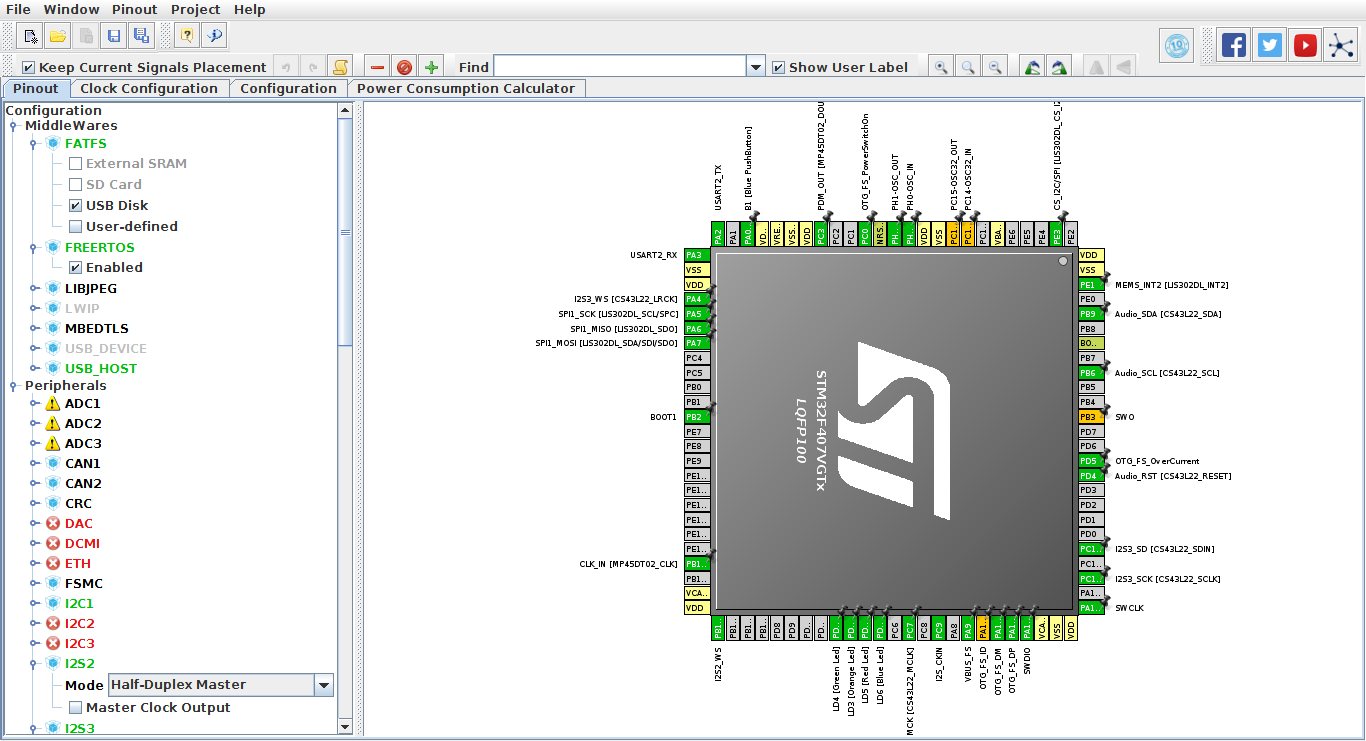
\includegraphics[width=\textwidth]{img/img1}}
 \caption{Konfiguracja \emph{FatFS}, \emph{FreeRTOS}, \emph{USB Host}, \emph{I2C1}, \emph{I2S2}}
 \label{img1}
\end{figure}

\begin{figure}[H]
 \centerline{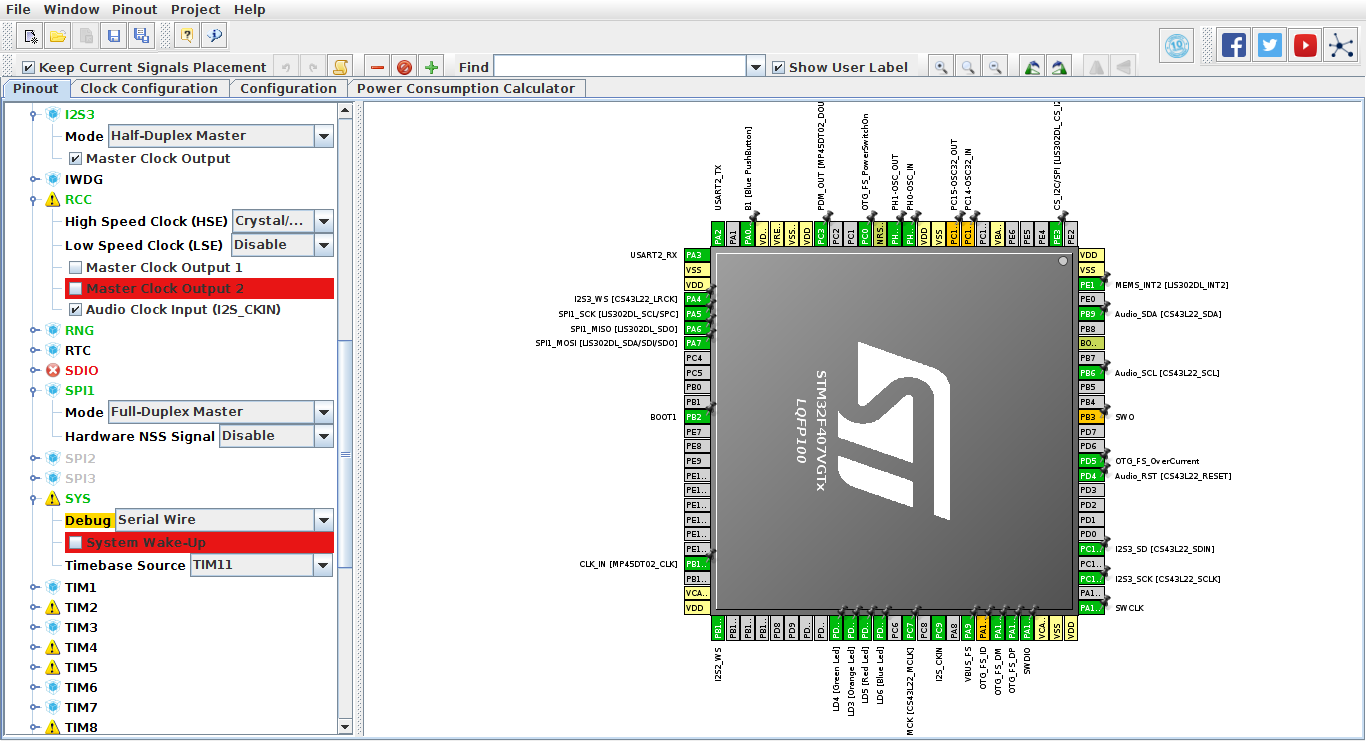
\includegraphics[width=\textwidth]{img/img2}}
 \caption{Konfiguracja \emph{I2S3}, \emph{RCC}, \emph{SPI1}, \emph{SYS}}
 \label{img2}
\end{figure}

\begin{figure}[H]
 \centerline{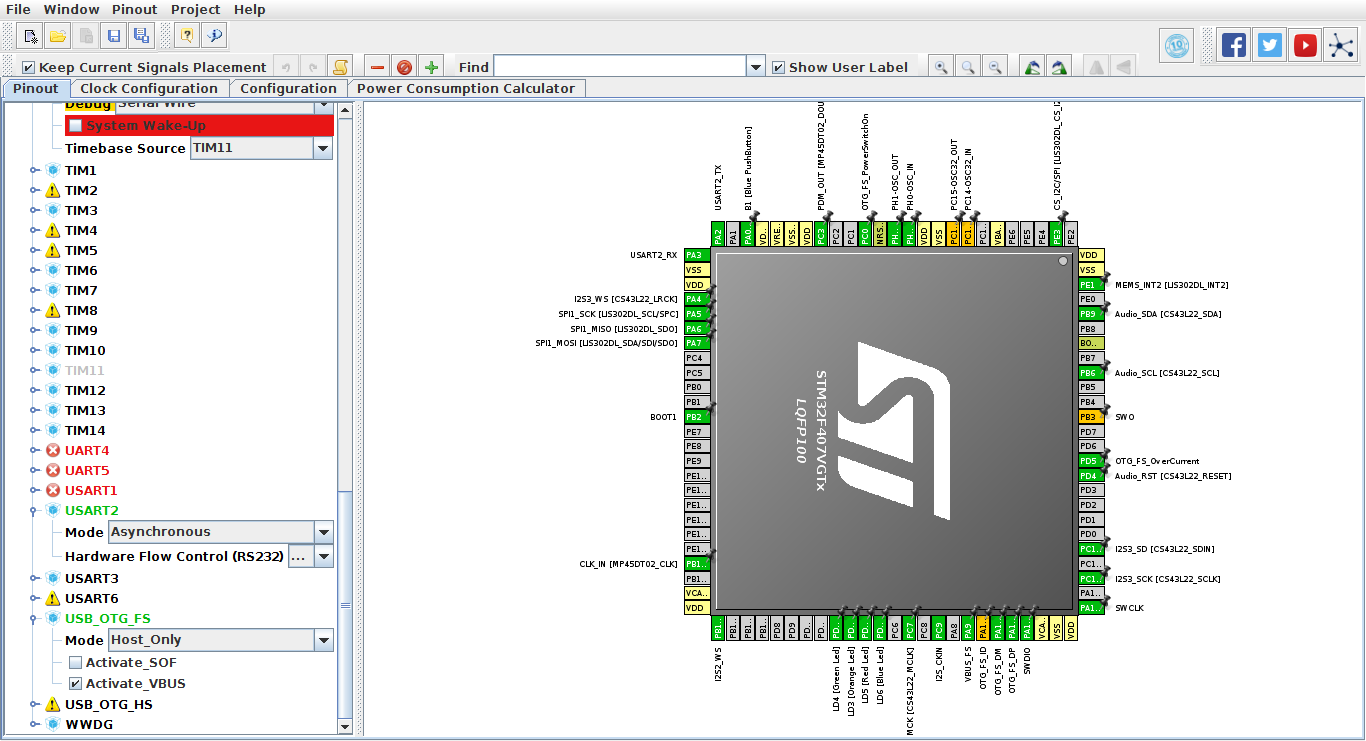
\includegraphics[width=\textwidth]{img/img3}}
 \caption{Konfiguracja \emph{USART2}, \emph{USB OTG FS}}
 \label{img3}
\end{figure}

\begin{figure}[H]
 \centerline{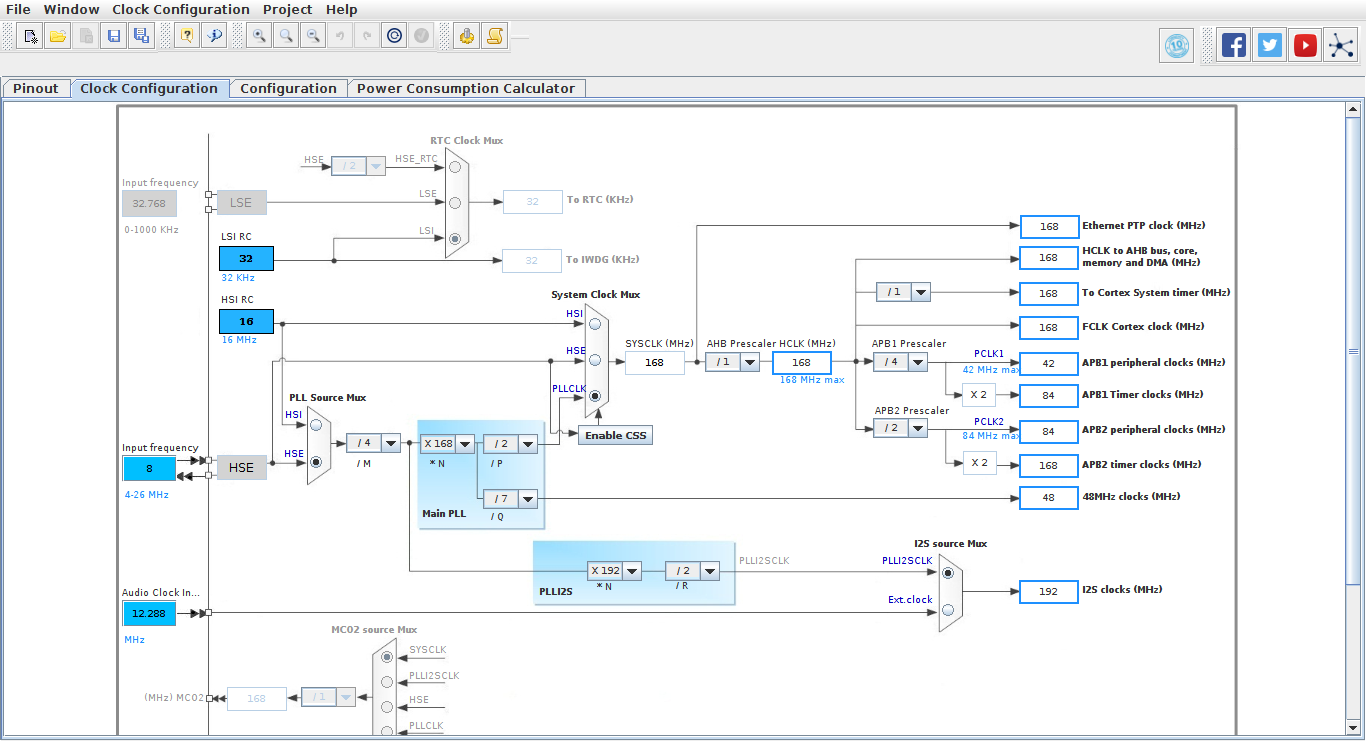
\includegraphics[width=\textwidth]{img/img4}}
 \caption{Konfiguracja zegara}
 \label{img4}
\end{figure}

\begin{figure}[H]
 \centerline{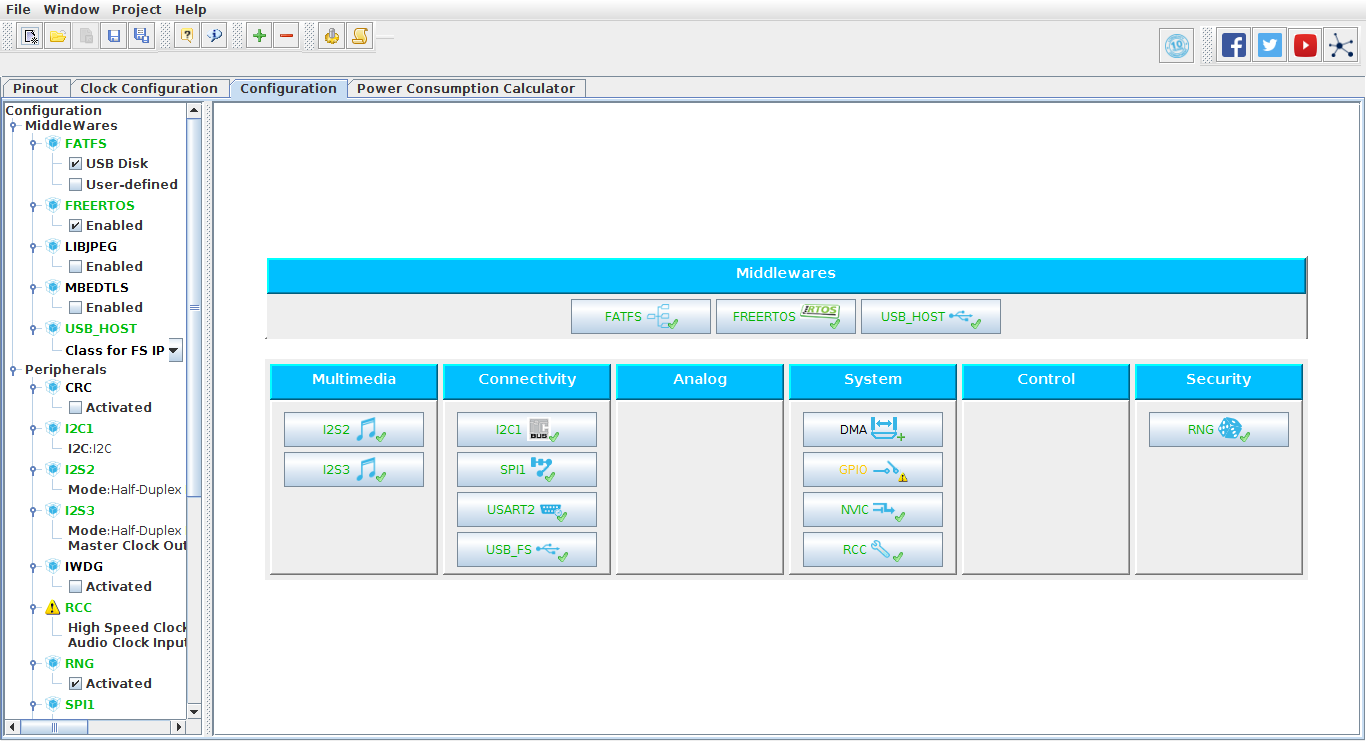
\includegraphics[width=\textwidth]{img/img5}}
 \caption{Podsumowanie konfiguracji}
 \label{img5}
\end{figure}

\section{\emph{Wave Player} -- przegląd kodu}

\subsection{Założenia projektu}
Ta wersja projektu ma za zadanie odtwarzanie pliku \emph{WAVE} o danej nazwie z podłączonej do płytki przez USB pamięci flash. Kolejne kroki wykonywane przez program to:
\begin{itemize}
 \item montowanie systemu plików,
 \item otwieranie pliku muzycznego,
 \item wczytywanie początku pliku do bufora,
 \item rozpoczęcie odtwarzania danych z bufora,
 \item uzupełnianie bufora w reakcji na przerwania,
 \item kończenie odtwarzania.
\end{itemize}

\subsection{Default Task (\emph{FreeRTOS})}

\begin{lstlisting}
/* StartDefaultTask function */
void StartDefaultTask(void const *argument) {
    /* init code for FATFS */
    MX_FATFS_Init();

    /* init code for USB_HOST */
    MX_USB_HOST_Init();

    /* USER CODE BEGIN 5 */
    osDelay(500);

    if (f_mount(&USBDISKFatFs, (TCHAR const *) USBDISKPath, 0) != FR_OK) {
        printf("f_mount FAILED\n");
    } else {
        printf("f_mount SUCCEDED\n");
        WavePlayerStart();
    }
    /* Infinite loop */
    for (;;) {
        osDelay(500);
    }
    /* USER CODE END 5 */
}
\end{lstlisting}

W głównym zadaniu systemu operacyjnego inicjalizujemy biblioteki \emph{FatFS} i \emph{USBhost}, a następnie montujemy system plików. Jeżeli ta operacja się powiodła, to przystępujemy to dalszej pracy.

\end{document}
